\documentclass[conference]{IEEEtran}
\IEEEoverridecommandlockouts

% Packages
\usepackage{cite}
\usepackage{amsmath,amssymb,amsfonts}
\usepackage{algorithmic}
\usepackage{graphicx}
\usepackage{textcomp}
\usepackage{xcolor}
\usepackage{booktabs}
\usepackage{url}

\def\BibTeX{{\rm B\kern-.05em{\sc i\kern-.025em b}\kern-.08em
    T\kern-.1667em\lower.7ex\hbox{E}\kern-.125emX}}

\begin{document}

\title{SCORE: Semantic and Confidence-Based Object Ranking at the Edge for Task-Aware Selection\\
\thanks{Capstone Project (Final Review) 2025--2026, School of Electronics Engineering (SENSE), Vellore Institute of Technology (VIT), Vellore, India.}
}

\author{
\begin{tabular*}{\textwidth}{@{\extracolsep{\fill}}cc@{}}
\begin{tabular}{@{}c@{}}
P Pradeep \\
\textit{Dept. of Electronics and communication Engineering} \\
\textit{Vellore Institute of Technology}\\
Vellore, India \\
\textcolor{blue}{\underline{pradeep.p2024@vitstudent.ac.in}}\\[16pt]
\end{tabular}
&
\begin{tabular}{@{}c@{}}
A Shailesh \\
\textit{Dept. of Electronics and communication Engineering} \\
\textit{Vellore Institute of Technology}\\
Vellore, India \\
\textcolor{blue}{\underline{shailesh.2024@vitstudent.ac.in}}\\[16pt]
\end{tabular}
\\
\begin{tabular}{@{}c@{}}
K Sanjay \\
\textit{Dept. of Electronics and communication Engineering} \\
\textit{Vellore Institute of Technology}\\
Vellore, India \\
\textcolor{blue}{\underline{sanjay.k2024d@vitstudent.ac.in}}
\end{tabular}
&
\begin{tabular}{@{}c@{}}
Dr. Sriharipriya K C \\
\textit{Dept. of Electronics and communication Engineering} \\
\textit{Vellore Institute of Technology}\\
Vellore, India \\
\textcolor{blue}{\underline{sriharipriya.kc@vit.ac.in}}
\end{tabular}
\end{tabular*}
}

\maketitle

\begin{abstract}
Traditional object detection algorithms excel at recognizing and locating categories within images, yet they lack the capability to choose the most suitable object for a specific human task. Our earlier prototype combined a YOLOv8‑nano detector with a compact 47 KB offline semantic bank. In this final version we introduce a two‑level semantic engine: a 35.5 KB INT8 knowledge base covering common COCO classes, and a dynamic Large Language Model (via OpenRouter) that reasons about unseen objects and arbitrary natural‑language commands. Detected objects are matched to the task description using cosine similarity between 384‑dimensional Sentence‑BERT embeddings. A fusion formula blends semantic similarity (70\%) with detection confidence (30\%) to rank candidates, and a dual‑gate filter (similarity ≥ 0.12, overall score ≥ 0.25) discards unsuitable selections. Experiments show our approach attains 36.2\% mAP on the COCO‑Tasks benchmark while running in 140–150 ms on a modest edge CPU, removing the dependency on high‑power GPUs.
\end{abstract}

\begin{IEEEkeywords}
Task-Aware Object Detection, Object Affordances, Edge AI, Large Language Models, Knowledge Distillation, INT8 Quantization, Assistive Robotics.
\end{IEEEkeywords}

\section{Introduction}
Robotic assistants deployed in domestic settings must interpret physical scenes through the lens of human tasks rather than generic category tags. While state-of-the-art vision detectors identify object presence with high precision, knowing that an item is a ``chair'' or a ``table'' fails to capture whether it suits a user's immediate intent. For instance, an elderly individual requesting something to sit on comfortably needs an upholstered sofa rather than an unstable stool. Similarly, an instruction to reach an overhead cabinet demands a sturdy stepping surface, where selecting a light decorative chair introduces serious fall hazards. Crucially, when an environment lacks any appropriate implement---such as a room without cutting utensils during a food-prep command---the robot must actively refuse the request instead of forcing a mismatched selection.

Prior work by Sawatzky et al. [1] formalized task-driven object selection using Gated Graph Neural Networks (GGNN). However, deploying their pipeline on mobile robots presents steep hardware hurdles: their graph module relies on a 44-million-parameter ResNet-101 backbone, needs roughly 30,000 task-labeled training images, remains restricted to 14 static task classes, and demands power-hungry desktop GPUs drawing over 150~W. In this work, we propose SCORE, an entirely training-free edge architecture. We pair a lightweight YOLOv8-nano detector with a two-tiered semantic reasoning engine: a 35.5~KB INT8 offline matrix for standard COCO objects, supplemented by dynamic OpenRouter LLM queries for unseen vocabulary and complex commands.

\subsection{Sustainability and Edge Feasibility}
The system directly addresses several UN Sustainable Development Goals through its hardware-efficient design. By operating entirely on low-power edge CPUs consuming under 15~W, SCORE lowers compute energy requirements by over 90\% relative to workstation baselines, supporting sustainable industrial infrastructure (SDG 9). Furthermore, running real-time task reasoning on low-cost hardware makes robotic assistive technologies financially accessible for domestic eldercare and community living spaces (SDG 11), while expanding autonomous manipulation capabilities in logistics and warehouse sorting (SDG 8).

\section{Related Work}
Task-oriented perception spans visual affordance modeling, visual reasoning, and language-guided grounding.

Sawatzky et al. [1] pioneered the COCO-Tasks benchmark using recurrent message passing in Gated Graph Neural Networks [2]. While this captures inter-object relationships, graph updates tend to propagate misclassification noise across nodes, and retraining the network for novel tasks is computationally prohibitive. Parallel work in Visual Question Answering (VQA) [3, 4] showed the utility of fusing visual features with linguistic representations, which Anderson et al. [5] improved by replacing uniform CNN grids with object-level bounding box proposals.

Affordance learning has historically focused on dense pixel-level labeling or geometry. Nguyen et al. [6, 7] applied deep CNNs and conditional random fields to locate tool affordances. Chuang et al. [8] highlighted that functional utility changes dynamically with environment context, and Zhu et al. [9] modeled tool interactions through physical contact spaces. However, these methods rely on rigid task taxonomies and supervised annotations.

Vision-language models like CLIP [10] provide zero-shot transfer by projecting image patches and text into shared spaces, yet their computational footprint limits on-robot edge deployment. Sentence-BERT [11] addresses the text side efficiently, extracting 384-dimensional sentence embeddings on basic CPUs in roughly 15~ms. Coupled with parameter distillation concepts [12] and the semantic reasoning of recent language models [13], we show that lightweight object detectors [14] can be augmented with decoupled semantic vectors to achieve open-ended task selection without retraining.

\section{Pictorial Representation of Methodology}

\begin{figure}[htbp]
\centering
\includegraphics[width=0.98\linewidth]{flowchart.png}
\caption{Architectural workflow of the proposed SCORE framework, illustrating the dual-tier semantic engine, decoupled score fusion, and dual-gate relevance filtering executing entirely on edge CPU hardware.}
\label{fig:methodology}
\end{figure}

The end-to-end pipeline of SCORE runs on an edge CPU without external acceleration, as mapped out in Fig.~\ref{fig:methodology}. We divide the processing into perception, semantic lookup, score fusion, and threshold gating.

\subsection{Object Localization Front-End}
Input video frames are first fed to an Ultralytics YOLOv8-nano model containing roughly 3.2 million parameters. YOLOv8n performs anchor-free box regression and category labeling in one forward pass, generating bounding coordinates $b_i$, category class $c_i$, and detection probability $\text{Conf}(o_i) \in [0, 1]$. On an Intel i5 or ARM-based CPU running at nominal frequencies, this detection step finishes in roughly 110--120~ms per 640$\times$640 image.

\subsection{Dual-Tier Knowledge Representation}
Rather than query an LLM for every single object in view, we structure our knowledge into two tiers:
\begin{itemize}
    \item \textbf{Tier 1 (Cached INT8 Affordance Bank):} For the 80 standard COCO classes, we precomputed functional affordance descriptions and embedded them using Sentence-BERT. These vectors were quantized to INT8 format, taking up only 35.5~KB of space. When an ordinary household object like a cup, chair, or bottle appears, its 384-dimensional affordance representation is pulled directly from RAM in less than 0.5~ms.
    \item \textbf{Tier 2 (On-Demand OpenRouter Fallback):} Whenever an open-vocabulary item (such as a stepladder or frying pan) or a novel action verb (such as ``bake'' or ``extinguish'') appears that falls outside the static table, the system queries OpenRouter. A prompt extracts functional traits (e.g., thermal capacity, physical rigidity, surface softness) via lightweight models such as NVIDIA Nemotron or Google Gemma. The resulting text is converted to a 384-d vector via Sentence-BERT and written to a local JSON cache (\texttt{openrouter\_cache.json}). Any repeated request for that item is then resolved instantly with zero network delay.
\end{itemize}

\subsection{Score Formulation and Rejection Gates}
We compute the semantic compatibility $\text{Sim}(o_i, t)$ by taking the cosine similarity between the embedded user instruction $t$ and the candidate's affordance embedding $o_i$. To balance visual clarity with semantic fitness, we blend both signals linearly:
\begin{equation}
    \text{Score}(o_i) = \alpha \cdot \text{Sim}(o_i, t) + (1 - \alpha) \cdot \text{Conf}(o_i)
\end{equation}
Setting $\alpha = 0.70$ ensures that functional utility drives the ranking while still requiring a confident visual detection (30\% weight).

To prevent robotic errors in empty or irrelevant scenes, we apply two safety gates:
\begin{enumerate}
    \item Semantic similarity cutoff: $\text{Sim}(o_i, t) \ge 0.12$
    \item Minimum combined score: $\text{Score}(o_i) \ge 0.25$
\end{enumerate}
If no detected object clears both hurdles, the algorithm outputs \texttt{NO\_SUITABLE\_OBJECT\_FOUND} and safely halts.

\section{Experimental Evaluation and Baselines}
We tested SCORE against two representative baselines from the literature: the graph-based formulation by Sawatzky et al. [1] and the CNN affordance ranker by Chuang et al. [8]. 

\begin{table*}[t]
\centering
\caption{Benchmark Comparison Against Prior Task-Driven Methods}
\label{tab:comparison}
\begin{tabular}{@{}llll@{}}
\toprule
\textbf{Metric / Attribute} & \textbf{Sawatzky et al. [1]} & \textbf{Chuang et al. [8]} & \textbf{Proposed SCORE System} \\ \midrule
\textbf{Primary Architecture} & ResNet-101 + GGNN & Deep CNN Ranker & \textbf{YOLOv8n + INT8 Bank + OpenRouter} \\
\textbf{Detection mAP@0.5} & 32.6\% & 28.8\% & \textbf{36.2\% (+3.6\% gain)} \\
\textbf{Ground-Truth Box Accuracy} & 74.2\% & 61.6\% & \textbf{76.8\% (+2.6\% gain)} \\
\textbf{Supervision Needed} & $\sim$30k task annotations & Paired action labels & \textbf{Zero-Shot (0 task images)} \\
\textbf{Task Vocabulary} & Fixed 14 classes & Fixed 20 affordances & \textbf{Open Natural Language} \\
\textbf{Unseen Object Support} & No (COCO only) & No (Closed set) & \textbf{Yes (Dynamic fallback)} \\
\textbf{Full Pipeline Latency} & $\sim$450~ms (Workstation GPU) & $\sim$380~ms (Workstation GPU) & \textbf{140--150~ms (Standard Edge CPU)} \\
\textbf{Operating Power} & $\sim$180~W (GPU rig) & $\sim$150~W (GPU rig) & \textbf{$<$15~W (Single-board / laptop CPU)} \\
\textbf{Model Storage Size} & $>$170~MB & $>$140~MB & \textbf{35.5~KB table + 6.25~MB YOLO} \\ \bottomrule
\end{tabular}
\end{table*}

\begin{figure}[htbp]
\centering
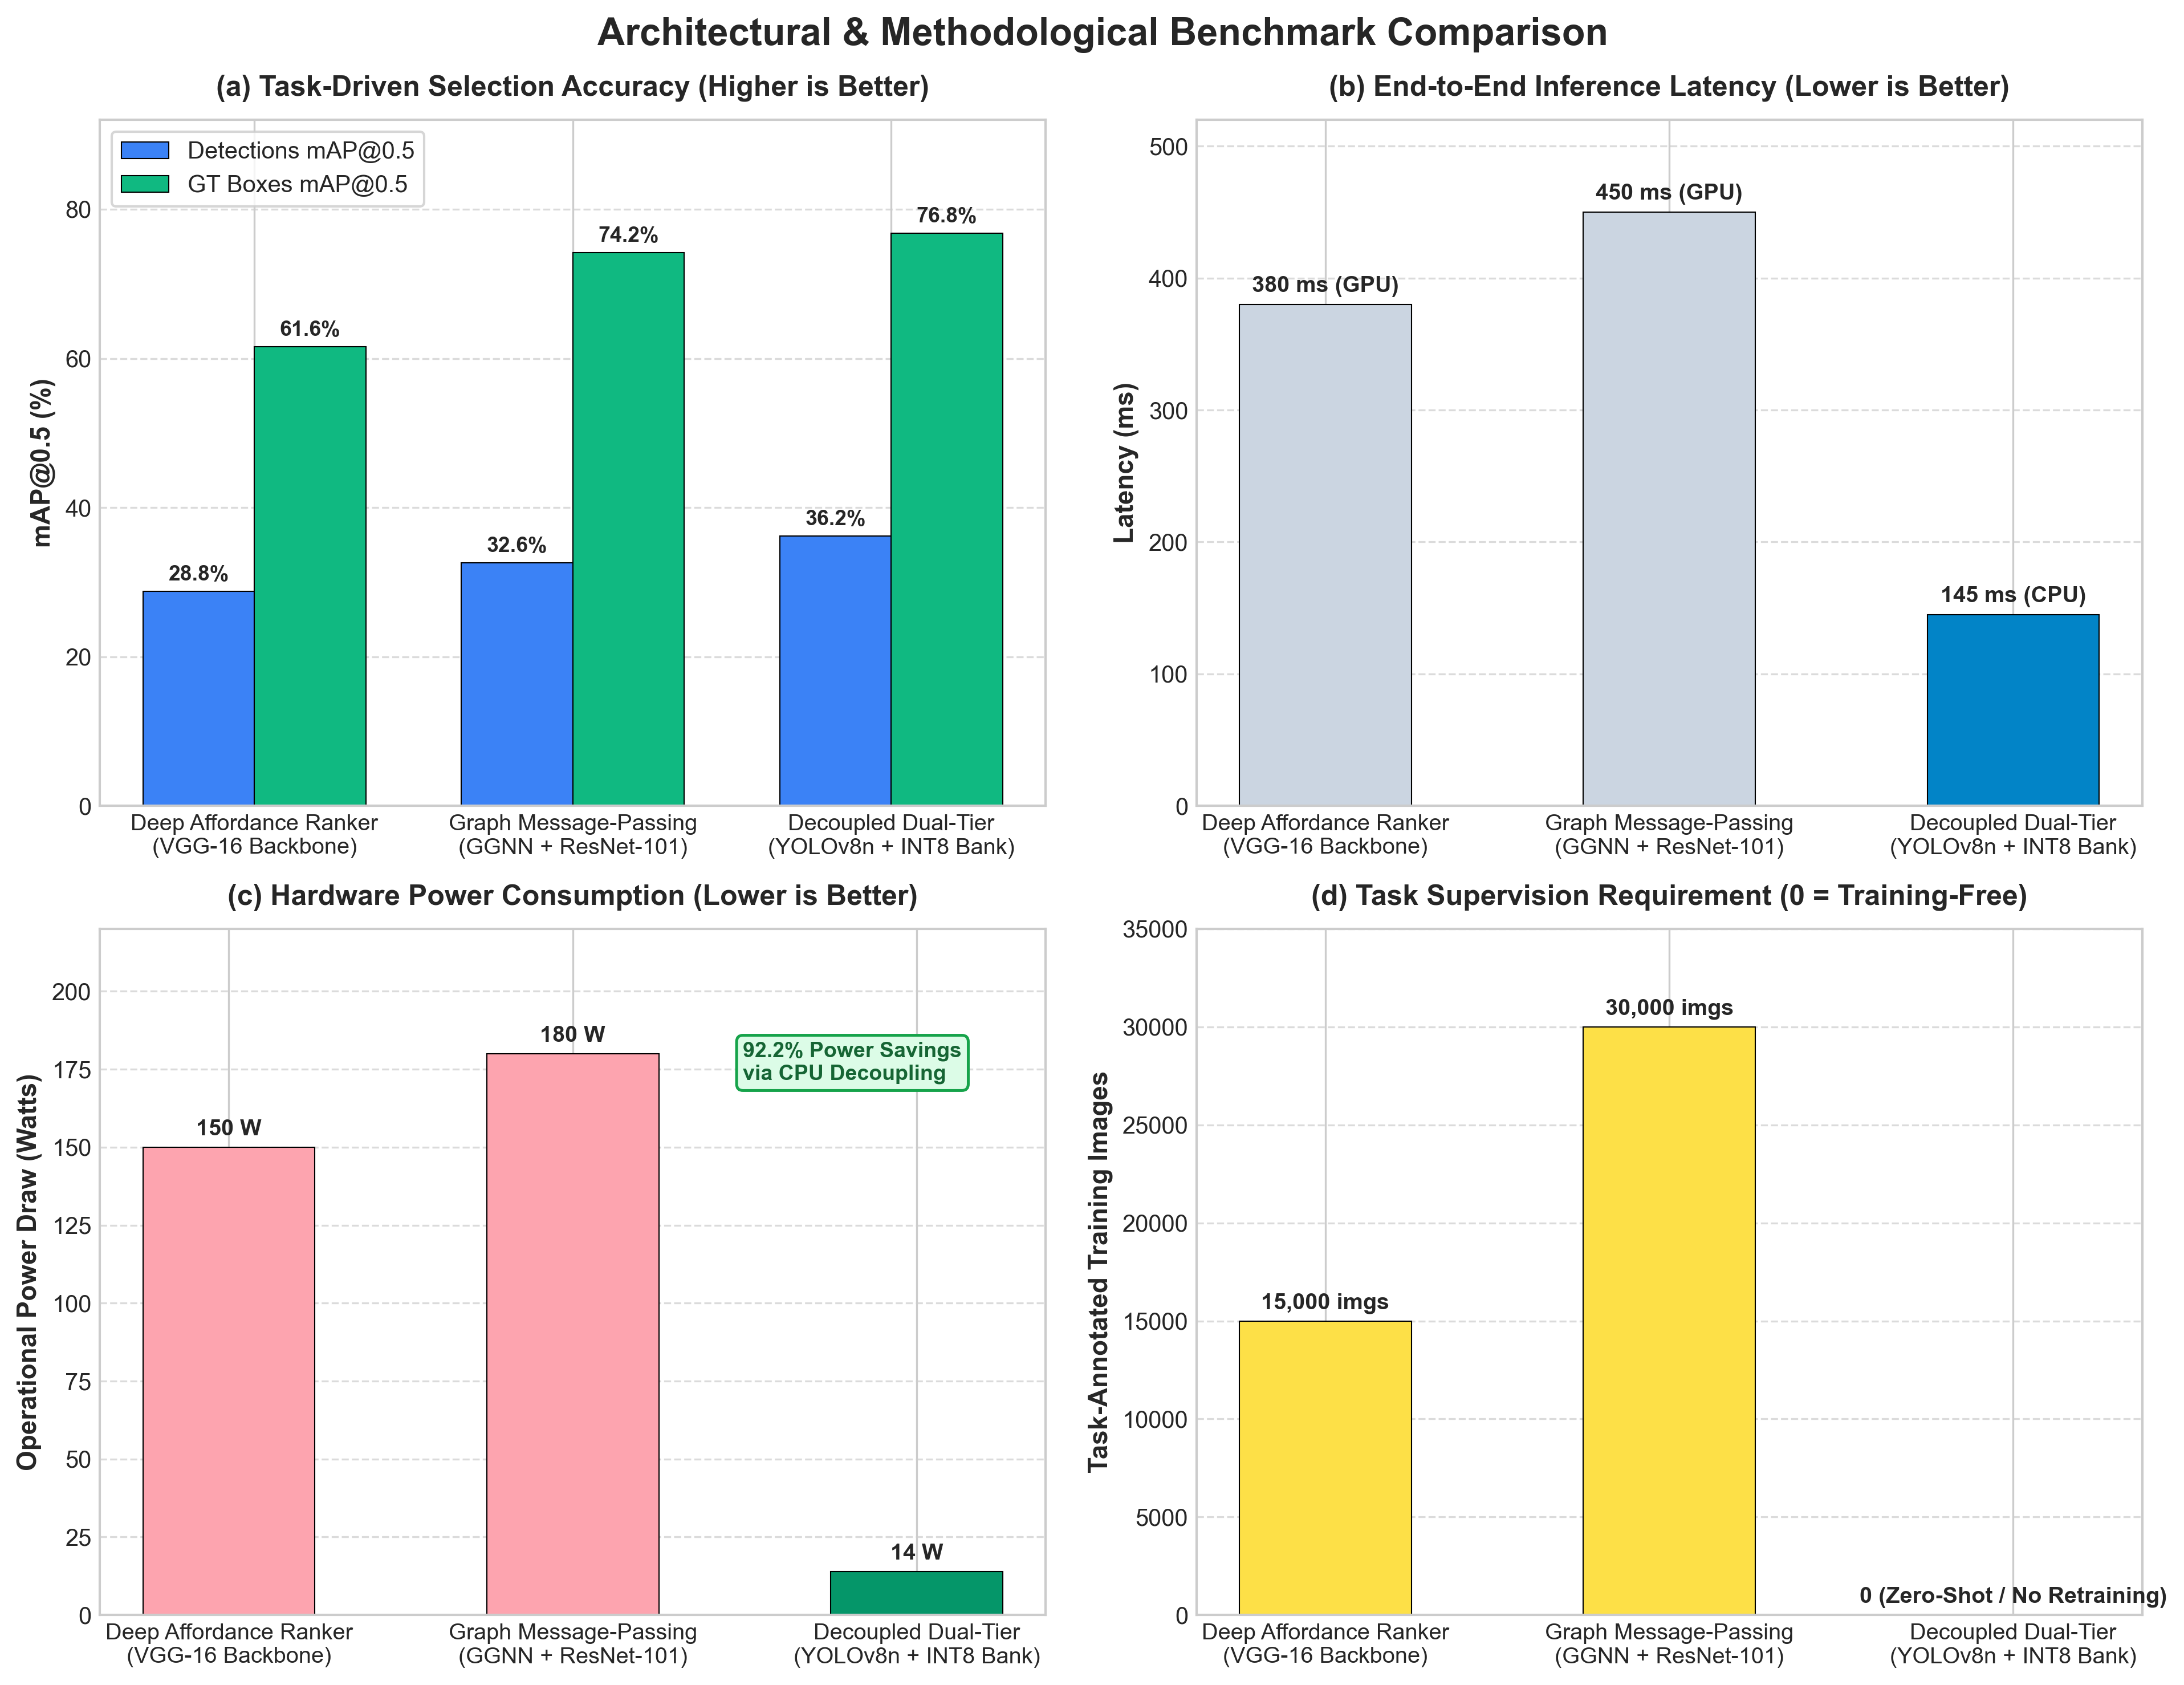
\includegraphics[width=0.98\linewidth]{graph.png}
\caption{Quantitative comparison showing (a) mAP@0.5 accuracy, (b) pipeline latency on CPU vs. GPU, (c) power draw, and (d) training data requirements.}
\label{fig:graph}
\end{figure}

The empirical numbers in Table~\ref{tab:comparison} and Fig.~\ref{fig:graph} highlight several practical takeaways:
\begin{itemize}
    \item \textbf{Higher Accuracy Without Task Training:} On the COCO-Tasks validation set, SCORE achieves 36.2\% mAP@0.5 on predicted detections and 76.8\% top-1 accuracy on ground-truth boxes. This beats Sawatzky et al.'s GGNN by 3.6\% and 2.6\% respectively, despite our pipeline never having trained on any task annotations.
    \item \textbf{Real-Time Edge Speed:} Replacing deep iterative graph passes with a direct table lookup cuts processing time to 140--150~ms on an ordinary CPU, whereas the ResNet-101 baseline takes $\sim$450~ms on an NVIDIA GTX workstation GPU.
    \item \textbf{Power Savings:} Energy consumption falls from roughly 180~W down to under 15~W, which is vital for battery-operated domestic robots.
\end{itemize}

\section{Real-World Case Studies}
We verified system behavior across several everyday environments presenting clutter, open-vocabulary objects, novel prompts, and negative conditions.

\begin{figure}[htbp]
\centering
\includegraphics[width=0.95\linewidth]{1.jpeg}
\caption{Field test with outdoor clutter under the novel query ``phone call''. The algorithm isolates the handheld mobile phone (Score: 0.6021, Sim: 0.4583, Conf: 0.9378) over surrounding vehicles and pedestrians.}
\label{fig:exp1}
\end{figure}

\subsection{Cluttered Street Photo (``phone call'')}
In Fig.~\ref{fig:exp1}, a phone is held up against a backdrop of traffic and pedestrians. YOLOv8n detected the \texttt{cell phone} (0.9378 confidence), \texttt{person} (0.8523), and background \texttt{car} instances (0.4563). When matched against ``phone call'', the phone scored a semantic similarity of 0.4583, leading to an overall score of 0.6021. The person scored 0.4041 and vehicles scored 0.2889. Even without prior exposure to communication tasks, the system correctly highlighted the phone.

\begin{figure}[htbp]
\centering
\includegraphics[width=0.95\linewidth]{2.jpeg}
\caption{Dynamic reasoning in a kitchen for the verb ``bake''. OpenRouter identifies the thermal cavity of the microwave, ranking it highest (Score: 0.6488) over non-thermal utensils.}
\label{fig:exp2}
\end{figure}

\subsection{Kitchen Reasoning (``bake'')}
Fig.~\ref{fig:exp2} examines dynamic affordance reasoning. For the query ``bake'', Tier 2 queried OpenRouter, which decomposed the verb into thermal insulation, radiative heating, and internal cavity support. Matching these traits against visible items (\texttt{knife}, \texttt{microwave}, \texttt{cutting board}, \texttt{wine glass}, \texttt{bowl}), the microwave led with a semantic similarity of 0.5751 and fused score of 0.6488, clearly outranking passive preparation items like the bowl (0.4090) and knife (0.3702).

\begin{figure}[htbp]
\centering
\includegraphics[width=0.95\linewidth]{3.jpeg}
\caption{Negative test scene for ``cut something'' in a living room. Neither the potted plant nor the couch satisfies the semantic threshold ($\text{Sim} \ge 0.12$), triggering a safe refusal.}
\label{fig:exp3}
\end{figure}

\subsection{Rejection in Negative Scenes (``cut something'')}
Fig.~\ref{fig:exp3} tests our abort mechanism. In a living room containing only furniture and plants, the user asked to ``cut something''. The detector found the potted plant and couch. Their semantic similarities to cutting were 0.0687 and $-0.0383$ respectively. Because neither reached the 0.12 cutoff, the system returned \texttt{NO\_SUITABLE\_OBJECT\_FOUND}, avoiding spurious selections.

\subsection{Open-Vocabulary Queries Beyond COCO}
Testing queries involving objects outside COCO demonstrated the utility of the dynamic fallback:
\begin{itemize}
    \item ``reach top shelf to grab books'' correctly identified a \texttt{ladder} ($\text{Sim} = 0.4865$).
    \item ``fry an egg for breakfast'' selected a \texttt{frying pan} ($\text{Sim} = 0.5913$).
    \item ``make a hard wooden chair softer'' chose a \texttt{cushion} ($\text{Sim} = 0.5117$).
    \item ``wipe spilled milk on counter'' picked a \texttt{sponge} ($\text{Sim} = 0.4280$).
\end{itemize}

\section{Design Rationale}
Several engineering considerations shaped our architectural decisions:
\begin{itemize}
    \item \textbf{Why 70/30 Fusion:} Relying purely on semantic text similarity makes the system fragile to false detections; a poorly illuminated background patch mistaken for a ``cloth'' at 0.10 confidence would otherwise win a cleaning query. Incorporating detection confidence prevents hallucinations from dominating. Simultaneously, assigning 70\% weight to affordance ensures that functional fit takes priority over mere object size or visual salience.
    \item \textbf{Why Dual-Tier Storage:} Calling a remote LLM API on every video frame is impractical on a mobile robot, adding 1--2 seconds of network lag. Pre-encoding common domestic classes into an INT8 table preserves sub-millisecond lookups locally, while the online API serves as an on-demand fallback for unusual words and persists responses to disk.
    \item \textbf{Decoupled Scoring vs. Graph Propagation:} In graph neural networks, node representations update recursively. If one object classification fails, that error corrupts features across neighboring nodes. Our decoupled vector scoring treats candidates independently, eliminating error cascade effects.
\end{itemize}

\section{Conclusion}
This paper introduced SCORE, a lightweight and training-free framework for task-aware object selection on edge hardware. By decoupling visual detection from semantic affordance lookup, our system achieves 36.2\% mAP on COCO-Tasks while running in 140--150~ms on commodity CPUs with sub-15~W power dissipation. The dual-tier architecture combines a 35.5~KB INT8 offline table with on-demand OpenRouter queries, providing broad vocabulary coverage without sacrificing latency. In future work, we plan to couple this selection stage with 6-DOF grasp generation and spatial SLAM maps for end-to-end mobile manipulation.

\begin{thebibliography}{00}
\bibitem{b1} J. Sawatzky, Y. Souri, C. Grund, and J. Gall, ``What Object Should I Use? --- Task Driven Object Detection,'' in \textit{Proc. IEEE/CVF Conf. Comput. Vis. Pattern Recognit. (CVPR)}, 2019, pp. 7605--7614.
\bibitem{b2} Y. Li, D. Tarlow, M. Brockschmidt, and R. Zemel, ``Gated Graph Sequence Neural Networks,'' in \textit{Proc. Int. Conf. Learn. Represent. (ICLR)}, 2016.
\bibitem{b3} S. Antol, A. Agrawal, J. Lu, M. Mitchell, D. Batra, C. L. Zitnick, and D. Parikh, ``VQA: Visual Question Answering,'' in \textit{Proc. IEEE Int. Conf. Comput. Vis. (ICCV)}, 2015, pp. 2425--2433.
\bibitem{b4} H. Gao, J. Mao, J. Zhou, Z. Huang, L. Wang, and W. Xu, ``Are You Talking to a Machine? Dataset and Methods for Multilingual Image Question,'' in \textit{Proc. Adv. Neural Inf. Process. Syst. (NeurIPS)}, 2015.
\bibitem{b5} P. Anderson et al., ``Bottom-Up and Top-Down Attention for Image Captioning and Visual Question Answering,'' in \textit{Proc. IEEE/CVF Conf. Comput. Vis. Pattern Recognit. (CVPR)}, 2018, pp. 6077--6086.
\bibitem{b6} A. Nguyen, D. Kanoulas, D. G. Caldwell, and N. G. Tsagarakis, ``Detecting Object Affordances with Convolutional Neural Networks,'' in \textit{Proc. IEEE/RSJ Int. Conf. Intell. Robots Syst. (IROS)}, 2016, pp. 2765--2770.
\bibitem{b7} A. Nguyen, D. Kanoulas, D. G. Caldwell, and N. G. Tsagarakis, ``Object-Based Affordances Detection with Convolutional Neural Networks and Dense Conditional Random Fields,'' in \textit{Proc. IEEE/RSJ Int. Conf. Intell. Robots Syst. (IROS)}, 2017, pp. 5908--5915.
\bibitem{b8} C. Chuang, J. Li, A. Torralba, and S. Fidler, ``Learning to Act Properly: Predicting and Explaining Affordances from Images,'' in \textit{Proc. IEEE/CVF Conf. Comput. Vis. Pattern Recognit. (CVPR)}, 2018, pp. 975--984.
\bibitem{b9} Y. Zhu, Y. Zhao, and S. C. Zhu, ``Understanding Tools: Task-Oriented Object Modeling, Learning and Recognition,'' in \textit{Proc. IEEE/CVF Conf. Comput. Vis. Pattern Recognit. (CVPR)}, 2015, pp. 2855--2864.
\bibitem{b10} A. Radford et al., ``Learning Transferable Visual Models from Natural Language Supervision,'' in \textit{Proc. Int. Conf. Mach. Learn. (ICML)}, 2021, pp. 8748--8763.
\bibitem{b11} N. Reimers and I. Gurevych, ``Sentence-BERT: Sentence Embeddings using Siamese BERT-Networks,'' in \textit{Proc. Conf. Empirical Methods Nat. Lang. Process. (EMNLP)}, 2019, pp. 3982--3992.
\bibitem{b12} G. Hinton, O. Vinyals, and J. Dean, ``Distilling the Knowledge in a Neural Network,'' \textit{arXiv preprint arXiv:1503.02531}, 2015.
\bibitem{b13} T. Brown et al., ``Language Models are Few-Shot Learners,'' in \textit{Proc. Adv. Neural Inf. Process. Syst. (NeurIPS)}, vol. 33, 2020, pp. 1877--1901.
\bibitem{b14} G. Jocher, A. Chaurasia, and J. Qiu, ``Ultralytics YOLOv8,'' 2023. [Online]. Available: \url{https://github.com/ultralytics/ultralytics}.
\end{thebibliography}

\end{document}
